\documentclass[Main]{subfiles} 
\begin{document}

\section{Designprocessen}
\begin{wrapfigure}{r}{0.6\textwidth}
	\vspace{-20pt}
	\centering
	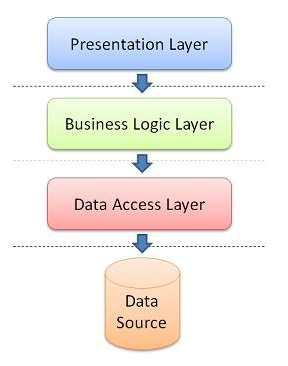
\includegraphics[scale=0.6]{Billeder/3-tier.png}
    \vspace{-15pt}
    \caption{3-Tier model}
  \label{fig:sprint1}
  \vspace{-10pt}
\end{wrapfigure}

Da udkastet til en kravspecifikation var f�rdig, skulle der naturligvis fasts�ttes nogle rammer for, hvordan systemearkitekturen skulle v�re. 
Det overordnede design blev fastlagt som det f�rste. 
Der var flere overvejelser og diskussioner om dette design, da det danner grundlag for hele systemet.
3-Tier modellen endte med at blive valgt som model for systemet (se figur \ref{fig:sprint1}).
\\
Denne model blev fundet simpel og solid, hvilket er to egenskaber der er blevet prioriteret h�jt i systemet. Grundid�en i modellen er at opdele systemet i uafh�ngige moduler, og som f�lge af det, vil der komme en lav afh�ngighed samt en h�j samh�righed, hvilke er m�l, der tilstr�bes i ethvert it-system. Dette resulterer ogs� i at et lag, som for eksempel gr�nsefladen, kan udskriftes, uden at hele systemet skal �ndres. Disse elementer samt simpelheden gjorde, at valget af den overordnede model faldt p� 3-Tier modellen.\footnote{Se afsnit \textit{5 LOGISK VIEW} i systemarkitekturdokumentet, for en detaljeret model af systemt}


Da 3-Tier modellen blev valgt, var der ikke mange overvejelser omkring, hvilken model brugergr�nsefladen skulle udvikles efter. MVVM er et meget benyttet m�nster inden for WPF, og er ogs� blev benyttet til opbygning af dette systems brugergr�nseflade. Opdeling af logikken og det grafiske, samt binding imellem disse, stemmer godt overens med 3-Tier modellen, hvilket ogs� er hovedgrunden til at dette m�nster er valgt. Derudover sikres en god opdeling af koden til brugergr�nsefladen med dette m�nster, og det grafiske kan dermed for eksempel nemt skiftes ud. Det opretholdes ved at GUI elementerne i Viewet's data er bundet til properties i MVVM's viewmodel og ikke hardcodet til modellen. Dermed er der kun afh�ngigheder nedad i systemet.
\\\\
Tilgangen til databasen, blev i f�rste omgang lavet som en ren tilgang. I videreudviklingen af denne tilgang, blev der diskuteret, hvilken metode der vil v�re bedst. Det endte ud med en beskedk�, hvor databasekaldene blev gemt. Denne k� underetter videre til databasetilgangs koden via \textit{observer}-m�nstret. K�en sikrer, at systemet kan k�re videre indtil databasen skal kontaktes, selvom forbindelsen til databasen skulle mistes. 
\\\\
I hele koden er der generelt gjort stor brug af interfaces. Dette er gjort, da interfaces g�r det nemt at teste kode, og da interfaces bruges i forbindelse med mange forskellige designm�nstre\footnote{Se afsnit 10.2 Arkitektur m�nstre i systemarkitekturen for oversigt over designm�nstre.}, samtidig med, at det bliver muligt at skifte objekter ud p� run-time f.eks. vha. strategy m�nstret. Et andet eksempel p� et designm�nster, er singleton. Dette designm�nster sikrer at en bestemt klasse kun kan oprettes en gang, og dette er b.la. brugt p� klassen
RobotEvent.\footnote{Se afsnit 8.2.2 Komponent 2: Simulering i systemarkitekturen for information om klassen RobotEvent}
Flere klasser benytter denne, til at fort�lle, at der er sket en h�ndelse med robotten, men da der kun er en robot, skal det naturligvis sikres at samme objekt bliver benyttet.\\
I det hele taget er forskellige designm�nstre blevet benyttet, til at sikre en solid og god kode.
\\\\
De forskellige designl�sninger der undervejs er blevet overvejet og diskuteret, har gjort at et solidt, fleksibelt og vedligeholdelsesvenligt program s� vidt er opn�et.
\end{document}